\chapter{Спектрально-аналитический метод поиска неточных повторов} \label{chapt2}
В работе исследуется спектральный метод поиска повторов в последовательностях
ДНК предложенный и разработанный коллективом кафедры математических методов
прогнозирования и института математических проблем в биологии Российской академии
наук (Пущино).

\bigskip
Метод разбивается на четыре основных этапа:
\begin{enumerate}
  \item Получение профилей последовательностей
  \item Спектральное индексирование полученных профилей
  \item Сравнение коэффициентов спектрального разложения
  \item Формирование матрицы гомологии
\end{enumerate}

\section{Профили последовательностей ДНК} \label{sect2_1}

Одной из главных особенностей рассматриваемого метода поиска повторов является
то, что на первом этапе последовательность преобразуется из дискретной в непрерывную
область. Это достигается построением т.н. профилей.

\bigskip
Под GC-профилем последовательности $X = (x_n)_{n=1}^{N_x}$ с окном $w$ в дальнейшем
будем понимать такую последовательность $P_{GC}(X,w)=(p_n^{GC})_{n=1}^{N_p},
N_p=N_x-w+1$, что 
$$
p_i^{GC}=\sum_{k=i}^{i+w}I^{GC}(x_k), i=\overline{1,N_p}
$$

где
$$
I^{GC}=
\left\{
  \begin{array}{rl}
    1,~x_n \in \{G,C\} \\
    0,~$иначе$ \\
  \end{array}
\right.
, n = \overline{1,N_x}
$$

\bigskip
Понятие GA-профиля определяется аналогично:
$$
P_{GA}(X,w)=(p_n^{GA})_{n=1}^{N_p}:
p_i^{GA}=\sum_{k=i}^{i+w}I^{GA}(x_k), i=\overline{1,N_p},
$$
где
$$
I^{GA}=
\left\{
  \begin{array}{rl}
    1,~x_n \in \{G,C\} \\
    0,~$иначе$ \\
  \end{array}
\right.
, n = \overline{1,N_x}
$$

\section{Спектральное индексирование профилей} \label{sect2_2}

На этом этапе профили переводятся в спектральное представление с использованием
в качестве базиса полиномов Чебышева дискретного аргумента или функций Фурье.

Под спектральным представлением сигнала $P=(p_n)_{n=1}^{N_p}$ будем понимать вектор
$\overline{C}=C_m(P)=(c_0,...,c_{m-1})$, где $c_0,...,c_{m-1}$ - первые $m$
коэффициентов разложения сигнала P по некоторой системе ортогональных функций
$u_0(x),...,u_{m-1}(x),...$
В случае использования в качестве базиса функций Фурье имеем:
$$
\begin{array}{rl}
    u_0(x)=1, \\
    u_1(x)=\cos{x}, u_2(x)=\sin{x}, \\
    u_3(x)=\cos{2x}, u_4(x)=\sin{2x}, \\
    ... \\
\end{array}
$$

Полиномы Чебышева определяются при помощи рекуррентного соотношения:
$$
\begin{array}{rl}
    u_0(x)=1, \\
    u_1(x)=x, \\
    u_{n+1}(x)=2xu_n(x)-u_{n-1}(x)
\end{array}
$$

Вычисление коэффициентов разложения в обоих случаях выполняется по
рекуррентным соотношениям

Рекуррентная схема вычисления коэффициентов разложения профилей позволяет
хорошо использовать кэш-память процессора, что оказывает существенное влияние на
производительность алгоритма.

\section{Спектральное сравнение профилей} \label{sect2_3}

На этой стадии спектральное представление профилей используется для
производства сравнения на основе некоторого специально разработанного критерия.

Теперь можно ввести понятие расстояния редактирования для рассматриваемого
метода поиска повторов.

Пусть $X_1,X_2$ - две последовательности ДНК, такие что $|X_1|=|X_2|=K \ge w$.
Будем понимать под GC- и GA-расстоянием редактирования для $X_1$ и $X_2$:
$$
\newcommand{\norm}[1]{\left\lVert#1\right\rVert}
\begin{array}{rl}
\rho^{GC}(X_1,X_2)= \norm{\overline{C_1^{GC}} - \overline{C_2^{GC}}}, \\
\rho^{GA}(X_1,X_2)= \norm{\overline{C_1^{GA}} - \overline{C_2^{GA}}}, \\
\norm{\overline{C}}=\sum_{i=0}^{m-1}c_i^2 \\
\end{array}
$$

под повтором будем понимать пару последовательностей $X_1,X_2$,
удовлетворяющих системе
$$
\left\{
  \begin{array}{rl}
      \rho^{GC}(X_1,X_2) < \epsilon \\
      \\
      \rho^{GA}(X_1,X_2) < \epsilon \\
  \end{array}
\right.
$$

\section{Построение матрицы гомологии} \label{sect2_4}
Под матрицей гомологии окном профилей w, окном аппроксимации a и шагом
аппроксимации s для последовательностей $X_1,X_2$ будем понимать матрицу
$$
\begin{array}{rl}
    M(X,Y,w,s,a)=(m_{ij})^{L_x*L_y}, \\
      \\
    L_x=[\frac{N_x-a-w+1}{s}],L_y=[\frac{N_y-a-w+1}{s}] \\
      \\
    m_{ij}=
    \left\{
      \begin{array}{rl}
        1,~x_n \in \{G,C\} \\
        0,~$иначе$ \\
      \end{array}
    \right.
\end{array}
$$

\bigskip
На рисунке \ref{img:gomology} приведена гомологическая матрица, образованная
в результате сравнения последовательности с самой собой. Матрица имеет
симметричный вид.
\bigskip

\begin{figure}[h]
\center{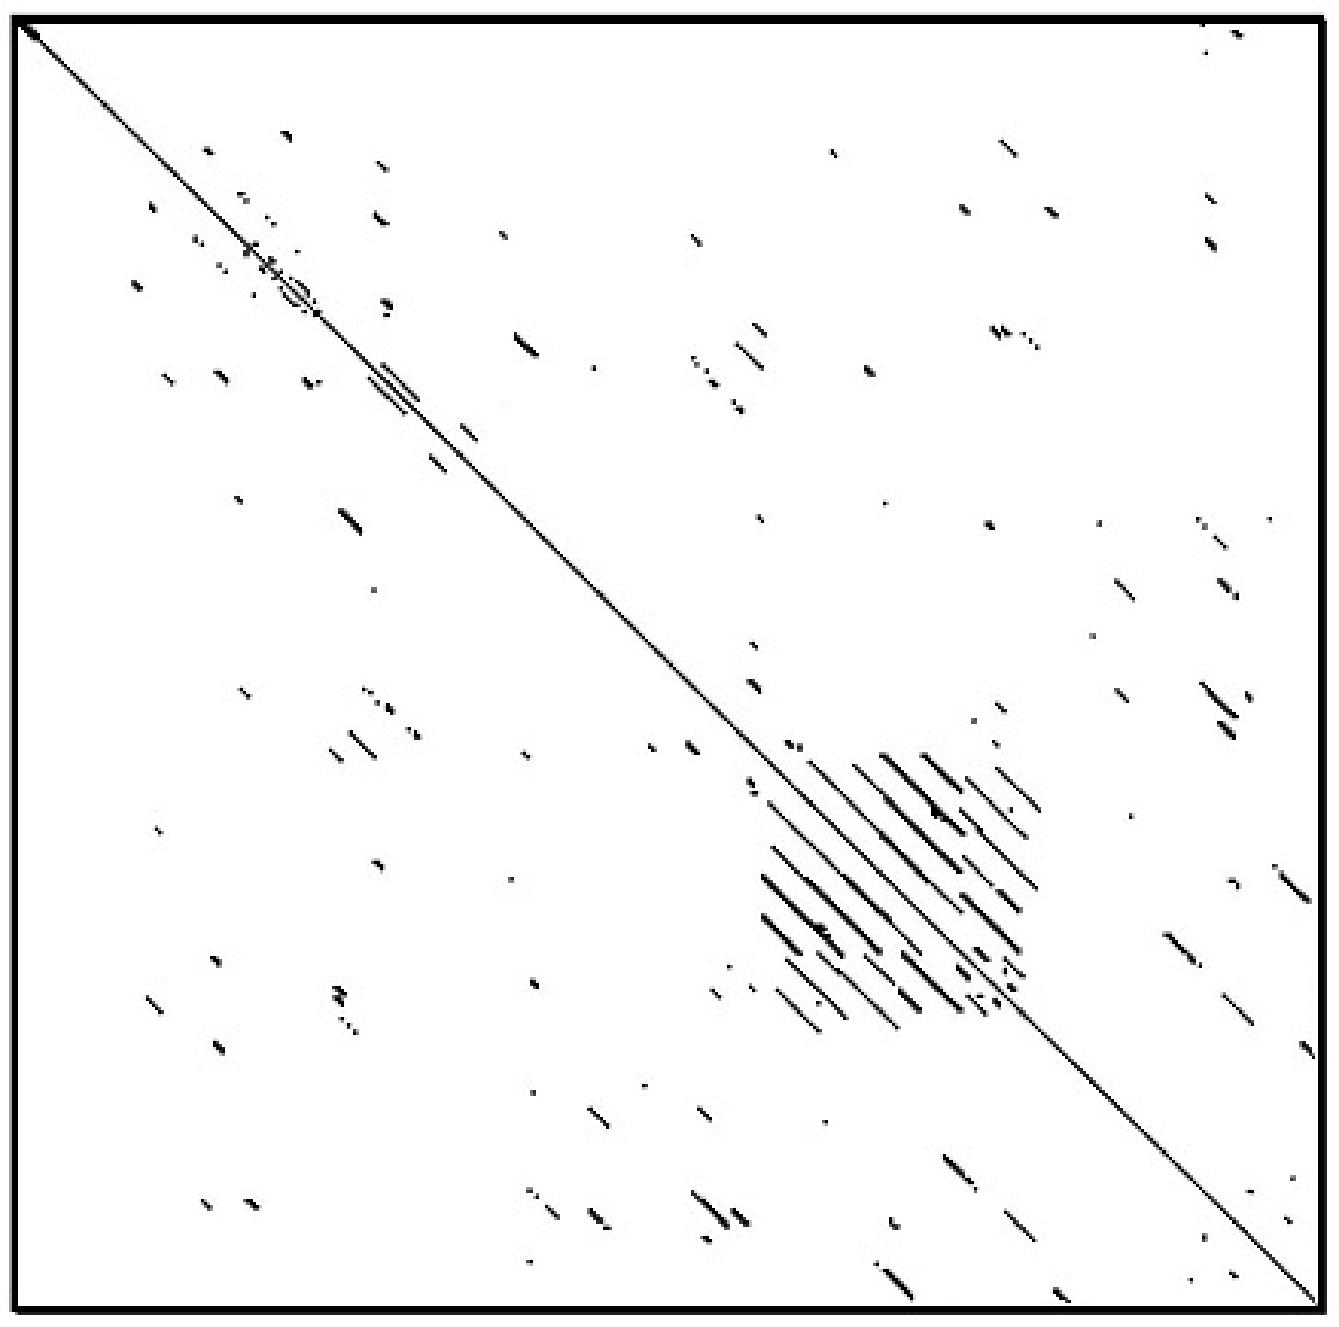
\includegraphics[width=0.5\linewidth]{image/0.jpg})}
\caption{Пример гомологической матрицы}
\label{img:gomology}  
\end{figure}

\clearpage
